% !TeX root = main.tex

\documentclass[10pt,aspectratio=169,dvipsnames]{beamer} % sets document type, default font size, slide aspect ratio, and loads color names
\usetheme[color/block=transparent]{metropolis} % sets the theme of the document

\usepackage[absolute,overlay]{textpos} % allows absolute positioning of text
\usepackage{booktabs} % enhances quality of tables
\usepackage[utf8]{inputenc} % allows input encoding in UTF-8
\usepackage{tikz} % used for creating vector graphics
\usetikzlibrary{arrows.meta} % loads additional arrow types
\usepackage[europeanresistors,americaninductors]{circuitikz} % for drawing electrical circuits
\usepackage[scale=2]{ccicons} % loads Creative Commons icons
\usepackage[official]{eurosym} % loads the official symbol for the Euro
\usepackage{fontawesome}
\usepackage[autostyle]{csquotes}
\usepackage{hyperref} % allows creating hyperlinks in the document
% \usepackage{emoji} 
\usepackage[absolute,overlay]{textpos} % Enable absolute positioning of elements
 

\newcommand{\ra}[1]{\renewcommand{\arraystretch}{#1}} % creates command to adjust spacing between rows
\newcommand{\hrefc}[2]{\href{#1}{\bf\color{blue}{\underline{#2}}}} % defines command for underlined, blue hyperlink
\newcommand{\urlc}[1]{\hrefc{#1}{#1}} % defines command for URL hyperlink

\newcommand{\R}{\mathbb{R}} % creates a shortcut for typing real numbers symbol
\newcommand{\ubar}[1]{\text{\b{$#1$}}} % defines a command for underlined text

\xdefinecolor{TUred}{RGB}{197,14,31} % defines a new color TUred
\setbeamerfont{alerted text}{series=\bfseries} % sets the font of alerted text to bold
\setbeamercolor{alerted text}{fg=TUred} % sets the color of alerted text to TUred
\setbeamercolor{background canvas}{bg=white} % sets the background color to white
\setbeamercolor{frametitle}{bg=lightgray!40, fg=TUred} % sets the background color of the frame title to light gray and text color to TUred
\setbeamercolor{title}{fg=TUred} % sets the color of the title to TUred

\addtobeamertemplate{frametitle}{}{% adds image to every frame title
  \begin{textblock*}{100mm}(1.01\textwidth,2pt)
    
\includegraphics[width=1.5cm]{images/TUB.png}
    \end{textblock*}}

\def\l{\lambda} % defines a shortcut for lambda symbol
\def\m{\mu} % defines a shortcut for mu symbol
\def\d{\partial} % defines a shortcut for partial symbol
\def\cL{\mathcal{L}} % defines a shortcut for caligraphic L symbol
\def\co{CO${}_2$} % defines a shortcut for CO2 symbol
\def\el{${}_{el}$} % defines a subscript for el
\def\th{${}_{th}$} % defines a subscript for th
\def\gas{${}_{gas}$} % defines a subscript for gas

\setbeamercolor{framesource}{fg=gray} % sets color of framesource to gray
\setbeamerfont{framesource}{size=\tiny} % sets font size of framesource to tiny
\newcommand{\source}[1]{% creates command for inserting a source footnote
\begin{textblock*}{5cm}(10.5cm,8.35cm)
    \begin{beamercolorbox}[ht=0.5cm,right]{framesource}
        \usebeamerfont{framesource}\usebeamercolor[fg]{framesource} {#1}
    \end{beamercolorbox}
\end{textblock*}}

\graphicspath{{../results/}} % sets the path where graphics can be found
\DeclareGraphicsExtensions{.pdf,.jpeg,.png,.jpg} % defines the types of graphic files that can be used

\def\goat#1{{\scriptsize\color{green}{[#1]}}} % defines a command for green, scriptsize text

\let\olditem\item % saves the old item command
\renewcommand{\item}{\olditem\vspace{5pt}} % redefines the item command to add space after each item


\title{Insights from model based studies \\ on 24/7 CFE and green hydrogen regulation}

%\subtitle{---}
\author{
  Elisabeth Zeyen \& Iegor Riepin\\
  \hrefc{mailto:e.zeyen@tu-berlin.de}{e.zeyen@tu-berlin.de} $\vert\vert$ 
  \hrefc{mailto:iegor.riepin@tu-berlin.de}{iegor.riepin@tu-berlin.de} \\
  Technical University of Berlin
  }

\date{DTU, 04 July 2024 \\

}

\usepackage{tcolorbox}
\usepackage[
type={CC},
modifier={by},
version={4.0},
]{doclicense}

\titlegraphic{%
  \vspace{0cm}
  \hspace{10.7cm}
    
\includegraphics[trim=0 0cm 0 0cm,height=1.2cm,clip=true]{images/TUB.png}
  \vspace{5.5cm}
  }

\setbeamertemplate{footline}{
	\usebeamercolor[fg]{framesource}%
	\usebeamerfont{page number in head}%
	\hspace{0.2cm}
	\small \insertframenumber
	\vspace{0.2cm}
	\scalebox{0.5}{\doclicenseIcon}
	\hfill
	%	
\includegraphics[height=0.8cm]{images/tublogo.pdf}
	%	\hspace{0.2cm}
}

% Disable the section title slides
\AtBeginSection[]{}
\setbeamercovered{transparent}

\setbeamertemplate{footline}[
myframe number]

% Change alert color to black
\setbeamercolor{alerted text}{fg=black}

% SOURCES
\setbeamercolor{framesource}{fg=gray}
\setbeamerfont{framesource}{size=\tiny}


% Redefine \sectionpage to only show the section name and not increment the frame counter
\makeatletter
\patchcmd{\sectionpage}{\usebeamertemplate*{headline}}{}{}{}
\patchcmd{\sectionpage}{\begin{center}\usebeamerfont*{section name}\insertsectionnumber.\ \end{center}}{}{}{}
\patchcmd{\sectionpage}{\begin{center}\usebeamerfont*{section title}\usebeamercolor[fg]{section title}\insertsectionhead\end{center}}{\begin{center}\usebeamerfont*{section title}\usebeamercolor[fg]{section title}\insertsectionhead\end{center}}{}{}
\makeatother

% Redefine \sectionpage to remove the section number
\def\sectionpage{\begin{centering}
		\begin{beamercolorbox}[sep=12pt,center]{part title}
			\usebeamerfont{part title}\insertsectionhead\par
		\end{beamercolorbox}
	\end{centering}
}

\usetheme[]{Berlin}

\begin{document}

\maketitle

%%%% 




% % Data centers work on technical solutions
% \begin{frame}{ICT companies work on concepts and technical solutions}

%   \begin{columns}[T]
%     \begin{column}{8cm}
%     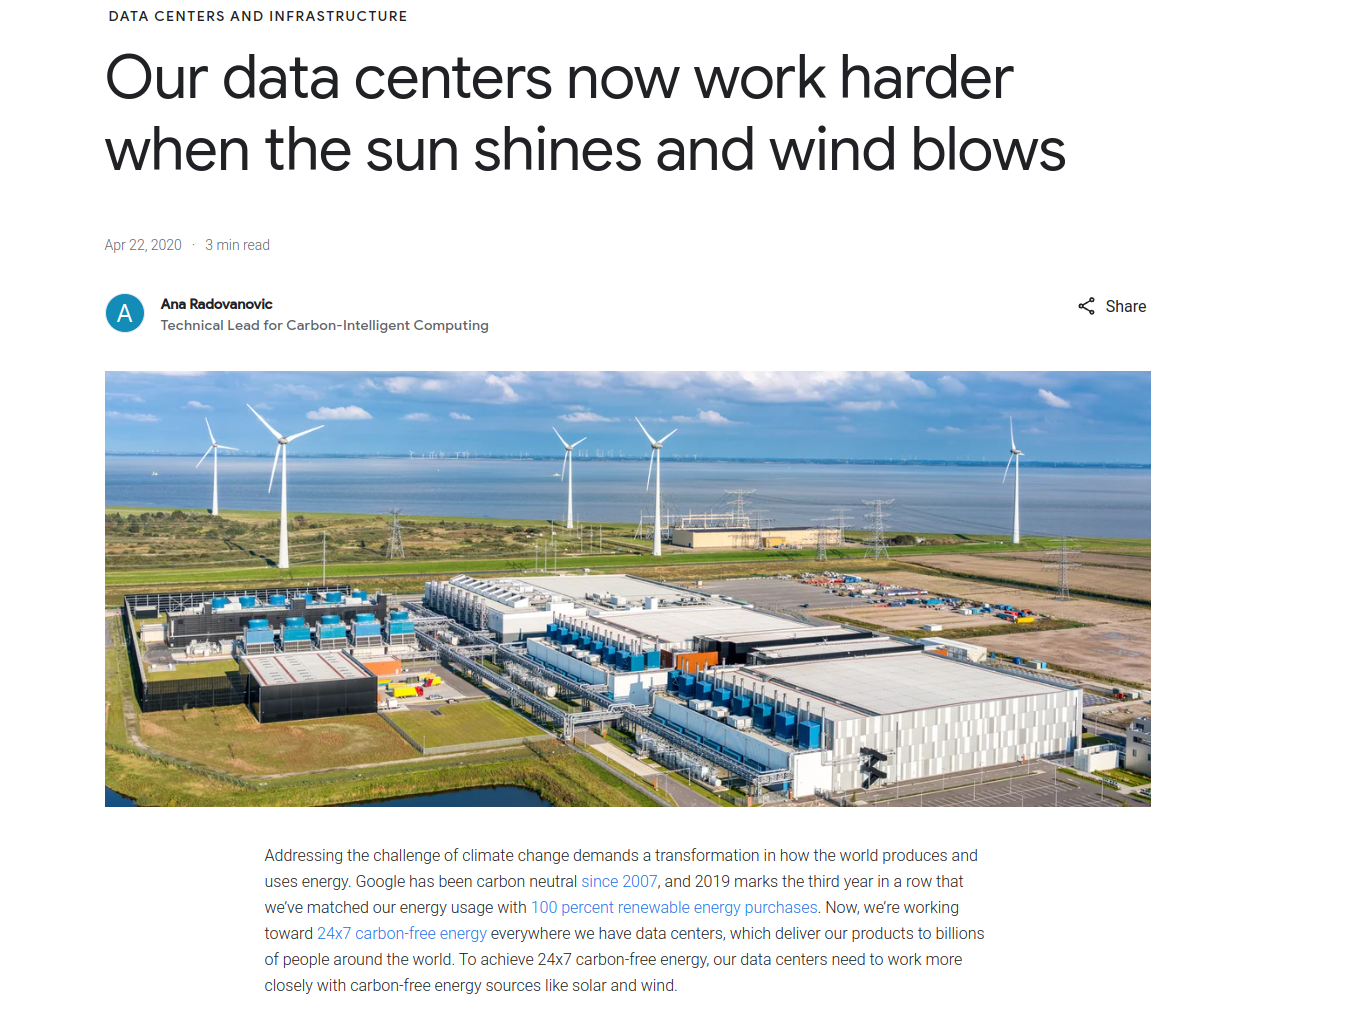
\includegraphics[width=9.1cm]{images/Radovanovic_blog.png}
%   \end{column}

%   \begin{column}{7cm}
%     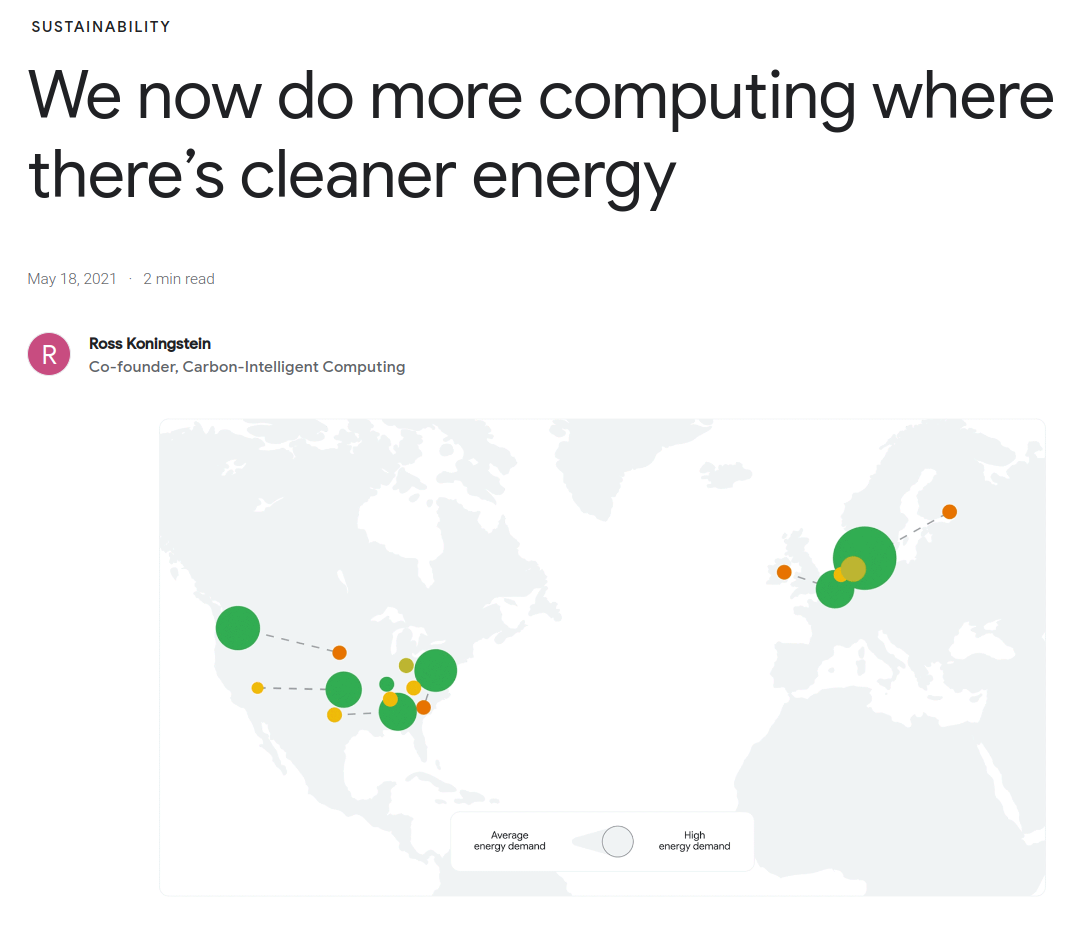
\includegraphics[width=7cm]{images/Koningstein_blog.png}
%     \source{
%       Sources: \\
%       \hrefc{https://blog.google/inside-google/infrastructure/data-centers-work-harder-sun-shines-wind-blows/}{blog.google/data-centers-work-harder-sun-shines-wind-blows} \\
%       \hrefc{https://blog.google/outreach-initiatives/sustainability/carbon-aware-computing-location/}{blog.google/carbon-aware-computing-location}}
% \end{column}

% \end{columns}
% \end{frame}

\section{Introduction}

\begin{frame}{Clean Electricity Procurement}
	\vspace{-1cm}
	\centering
	How to \alert{match} renewable generation with electricity demand?
	\vspace{0.5cm}
%		\begin{itemize}
%		\item A concept of \alert{hourly matching} got into the spotlight with debates on clean hydrogen regulation
%		\item Also a foundation for voluntary 24/7 carbon-free electricity (CFE) procurement  
%	\end{itemize}   
%		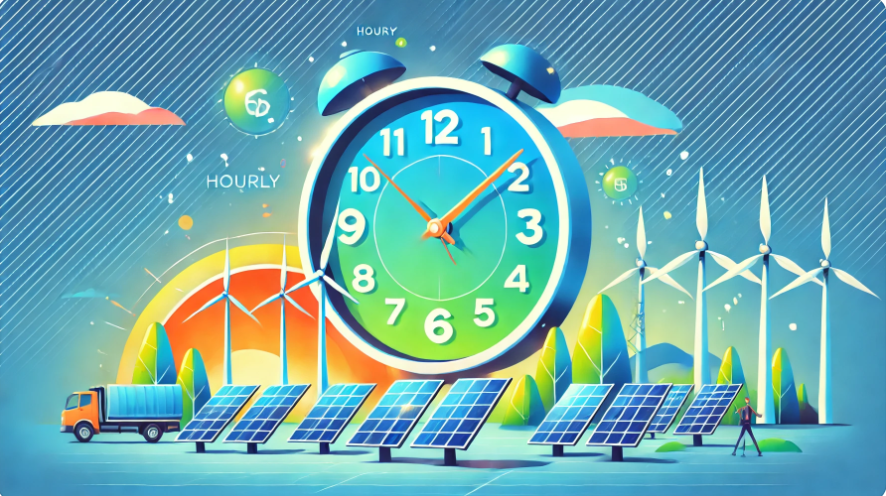
\includegraphics[width=0.7\linewidth]{images/hourly_electricity_procurement_v2}  
%	\source{ChatGPT4 hallucination, 2024}
	  \begin{columns}
		\begin{column}{0.4\textwidth}
		\begin{itemize}
			\item A concept of \alert{hourly matching} got into the spotlight with debates on clean hydrogen regulation
			\item Also a foundation for voluntary 24/7 carbon-free electricity (CFE) procurement  
		\end{itemize}      
		\end{column}
		\begin{column}{0.6\textwidth}
			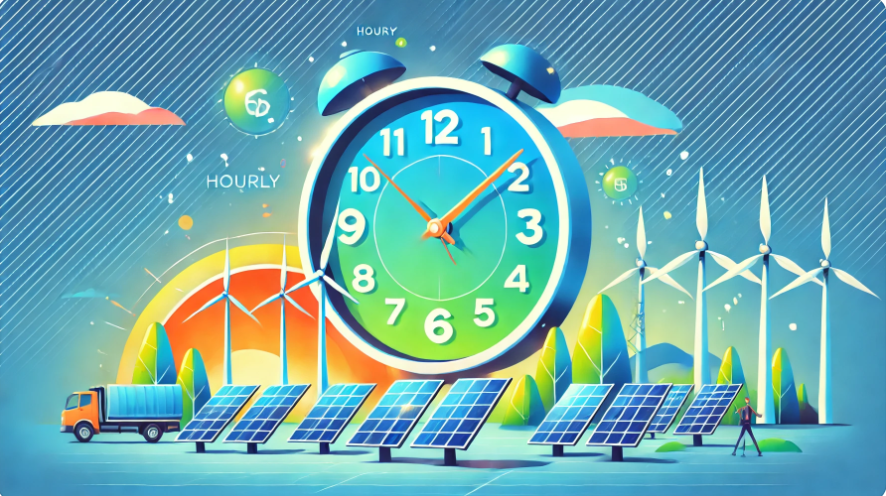
\includegraphics[width=1\linewidth]{images/hourly_electricity_procurement_v2}  
			\source{ChatGPT4 hallucination, 2024}	
		\end{column}
	\end{columns}
\end{frame}
\section{Temporal Regulation Green Hydrogen}
\begin{frame}[noframenumbering, plain]
	
	\begin{figure}
		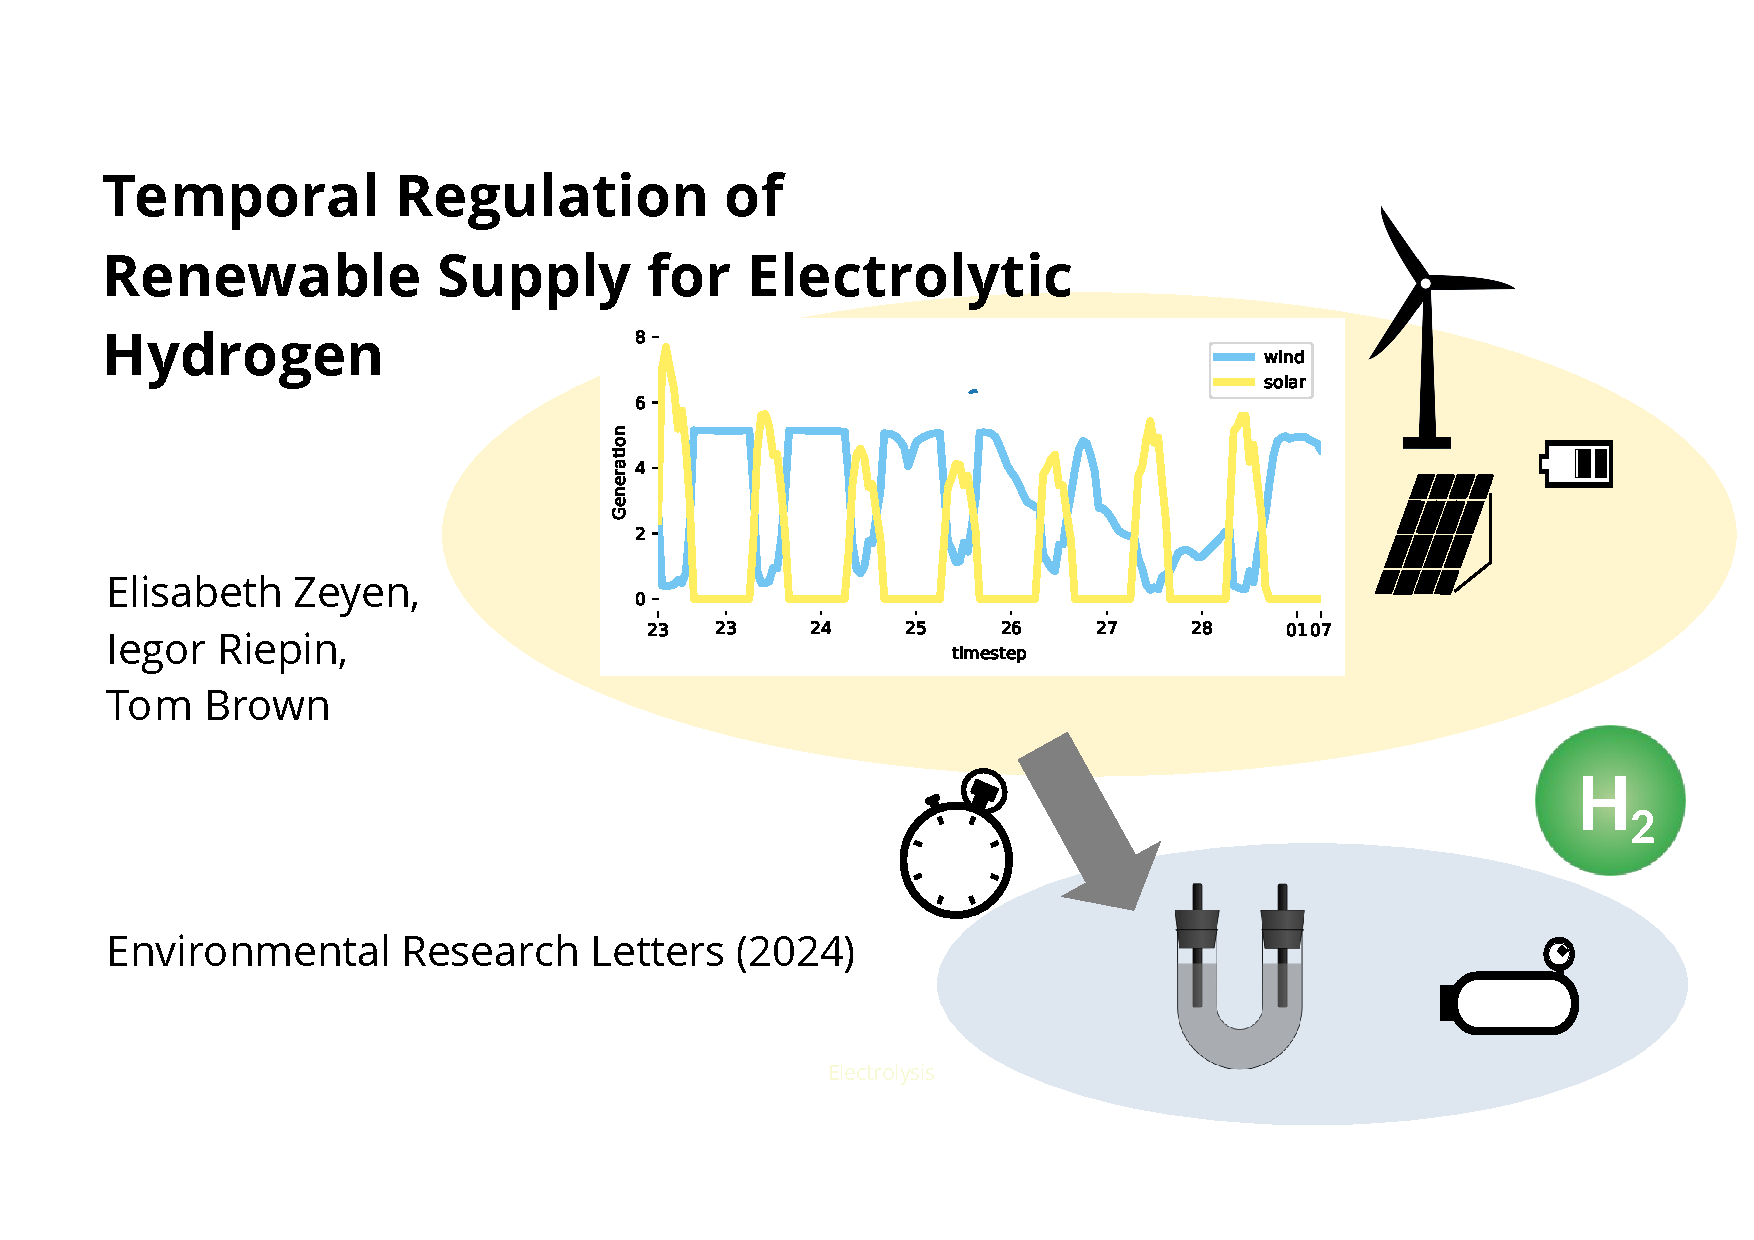
\includegraphics[trim={0cm 0cm 0cm 0cm}, width=0.9\linewidth]{images/titlepage_greenh2.pdf}
	\end{figure}
	
\end{frame}
\begin{frame}{Motivation - The Urgency of Green Hydrogen Standards}
	%	\alert{Background}: Green hydrogen can be used in sectors which are hard to decarbonise.  Thus, there's a need for clear standards defining 'green' hydrogen. \\
	\alert{Challenge}: Rapid scale up of affordable green hydrogen production without emissions increases. \\
	\alert{What happened so far}:
	\begin{itemize}
		\item Various standards are under discussion, differing in how strictly renewable generation must align with the electrolysis electricity demand.
		\item The EU adopted a Delegated Act in 2023, hourly matching from 2030 
		\\ $\rightarrow$ \alert{Delegated Act} is subject to \alert{review in July 2028}.
		%		\item Germany published its updated national green hydrogen strategy in July 2023
	\end{itemize} 
\end{frame}

\begin{frame}{Questions We Want to Answer in This Study}
	\begin{columns}[t]
		% Column 1
		\begin{column}{0.5\textwidth}
			\centering
			
\includegraphics[width=2cm]{images/globalwarming.png} \\
			How do \alert{various certification} standards affect \alert{emissions}?\\
		\end{column}
		
		% Column 2
		\begin{column}{0.5\textwidth}
			\centering
			
\includegraphics[width=2cm]{images/coin.png} \\
			How do regulations impact \alert{hydrogen production costs}?
		\end{column}
	\end{columns}
	\vspace{0.5 cm}
	\begin{tcolorbox}[colback=gray!5,colframe=white!60!black,title=\textbf{Scientific Novelty}]
		\alert{Quantify impact of individual modelling assumptions:} This includes hydrogen storage options, the background grid, and the methods used to model additionality.
	\end{tcolorbox}
\end{frame}


\begin{frame}{Methods - Modelling Hydrogen's Temporal Regulation}
	Hydrogen production in one selected European country with a \alert{constant} hydrogen demand of 28 TWh$_{\text{H}_2}$/a. 
	\begin{figure}
		\centering
		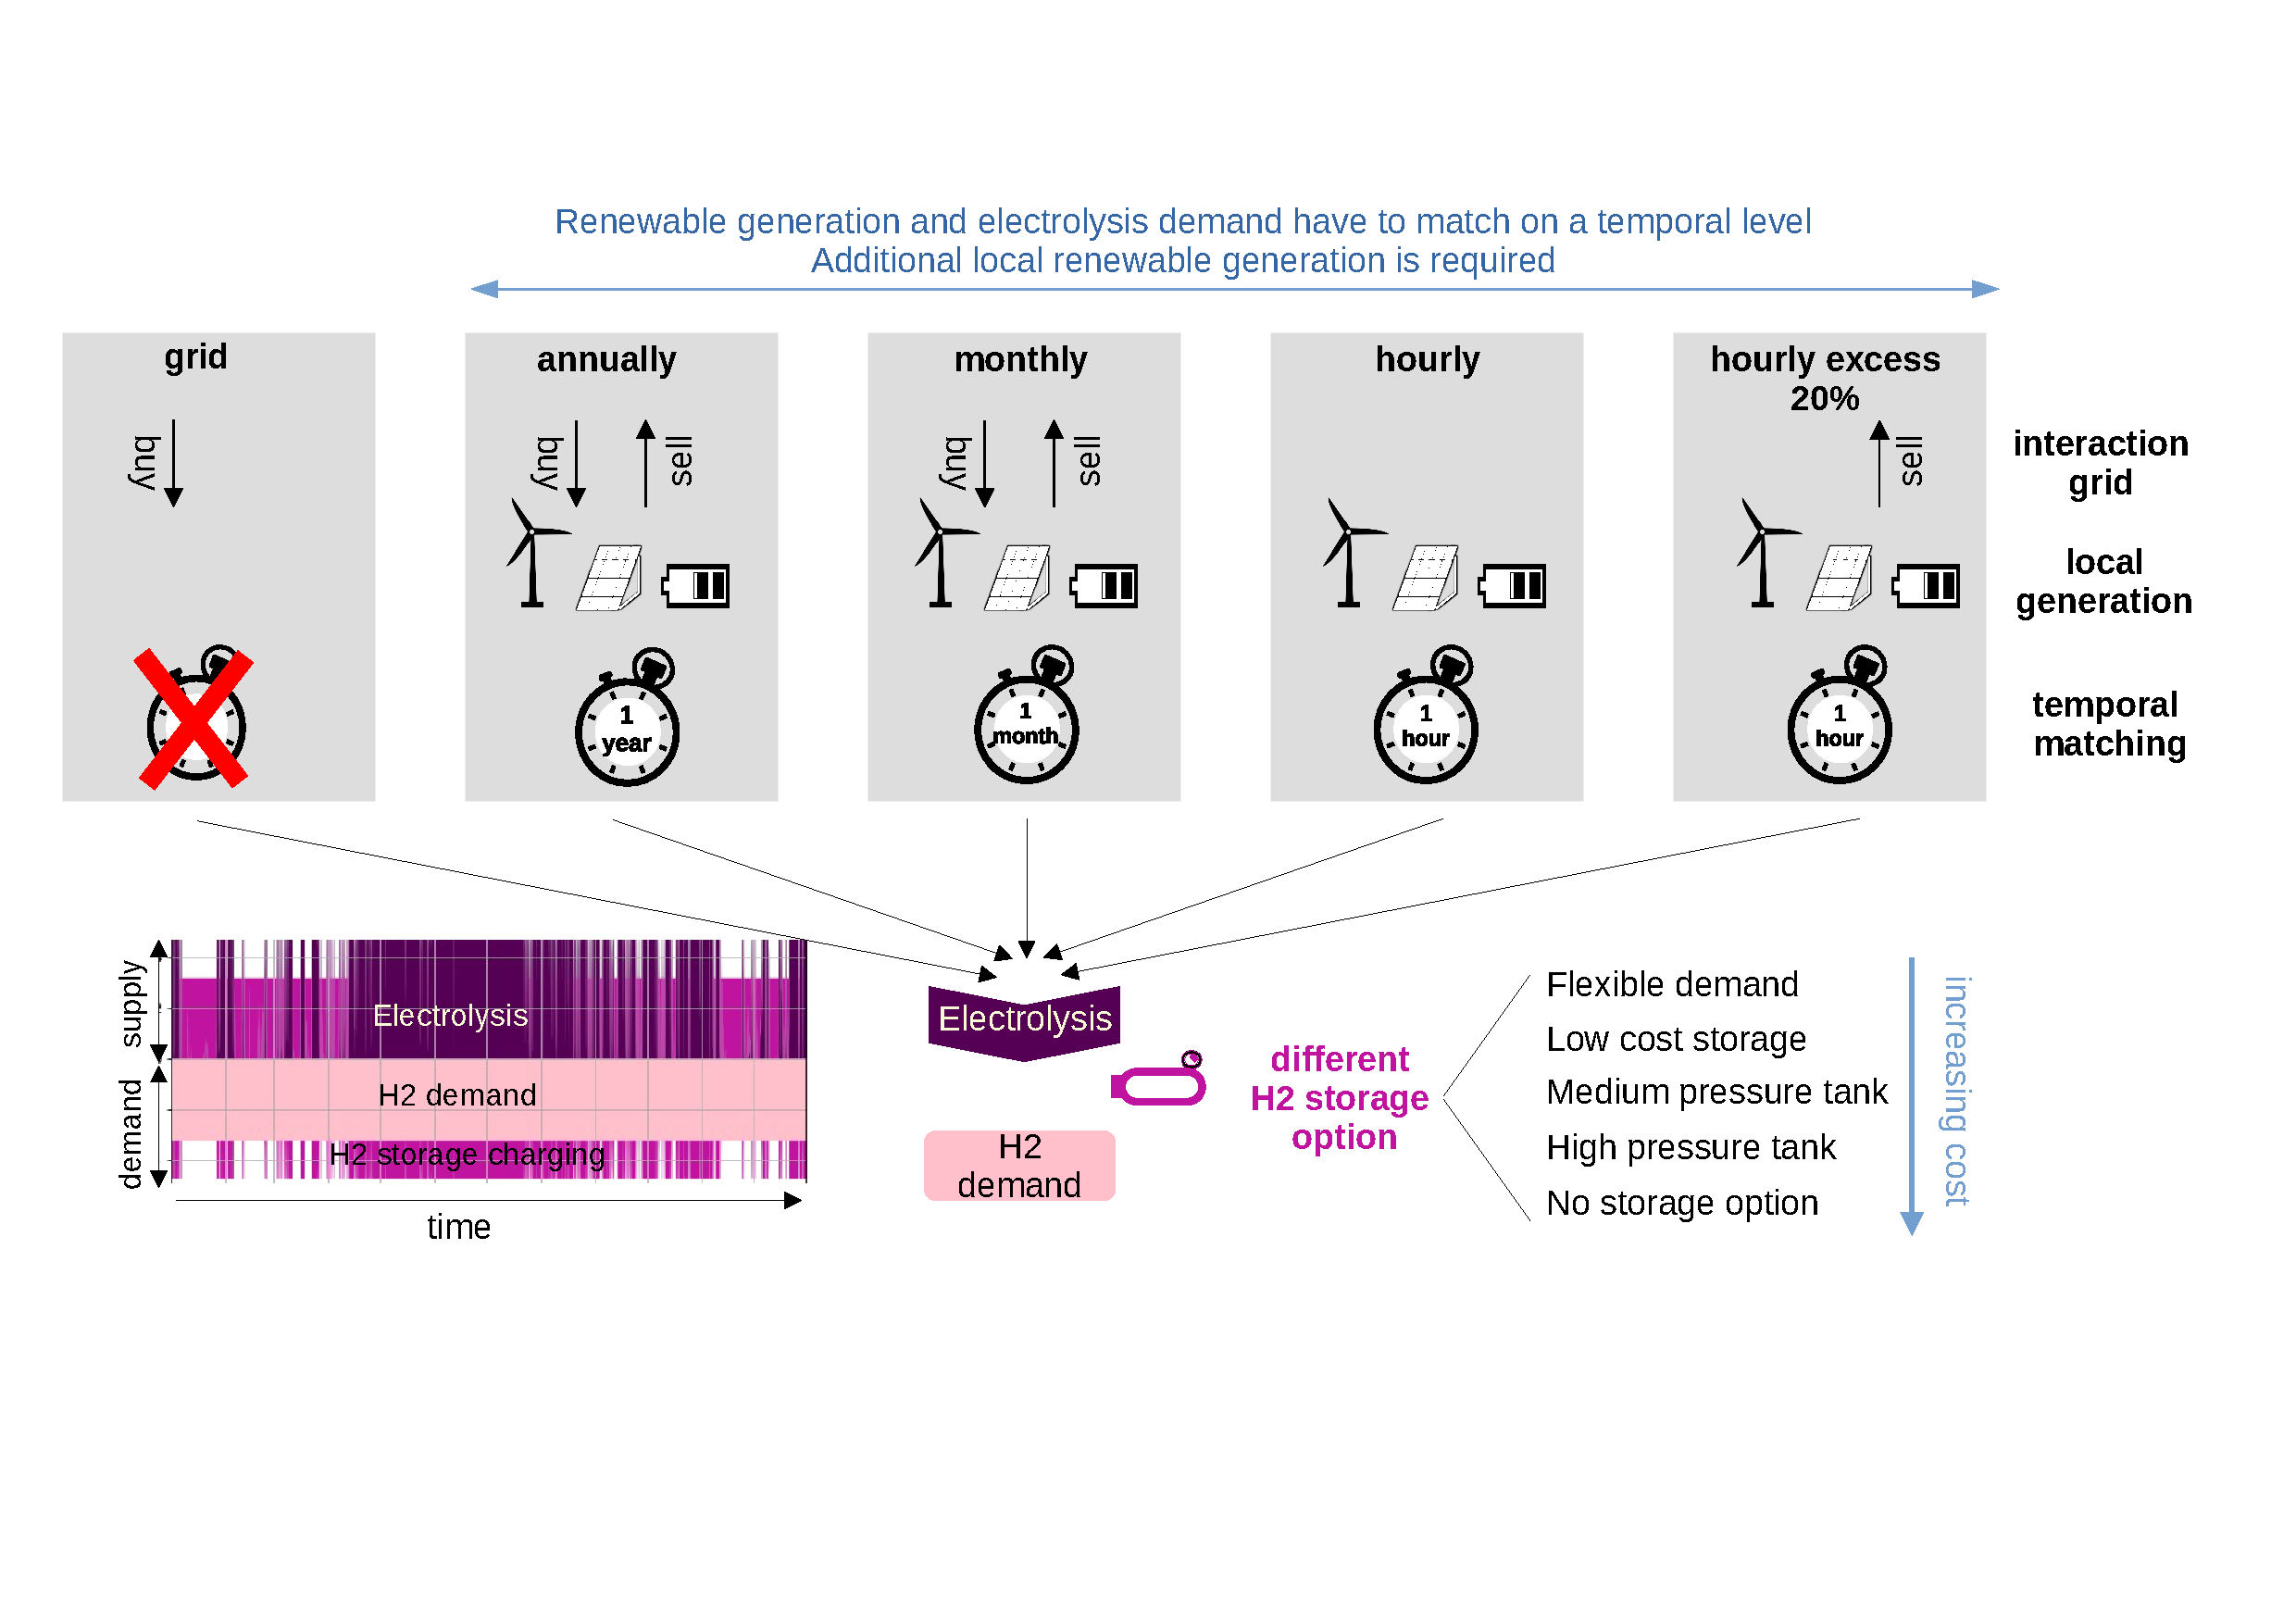
\includegraphics[trim=0 0cm 0cm 3cm,clip=true, width=0.9\linewidth]{images/scenarios_new5_revised}
	\end{figure}
	
\end{frame}

\begin{frame}{Results - Emission Impacts of Hydrogen Production: Germany 2025}
	\begin{figure}
		\centering
		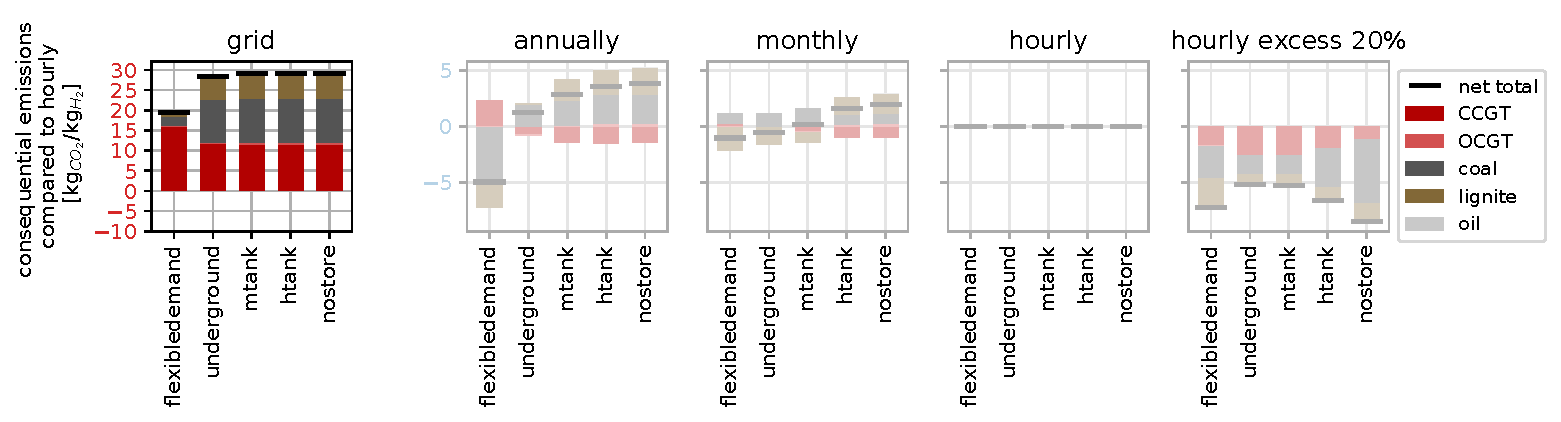
\includegraphics[width=1\linewidth]{images/consequential_emissions_by_carrier_3200wmonthly_v0.pdf}
	\end{figure}
	%To prevent emission increases, additional local procurement is essential. \\
	%The effects of annual vs. monthly matching are complex: flexible operations reduce emissions, but static operations increase them.\\
	%Hourly matching with excess sales offers the most significant emission reductions.
\end{frame}


\begin{frame}{Results - Emission Impacts of Hydrogen Production: Germany 2025}
	\addtocounter{framenumber}{-1}
	\begin{figure}
		\centering
		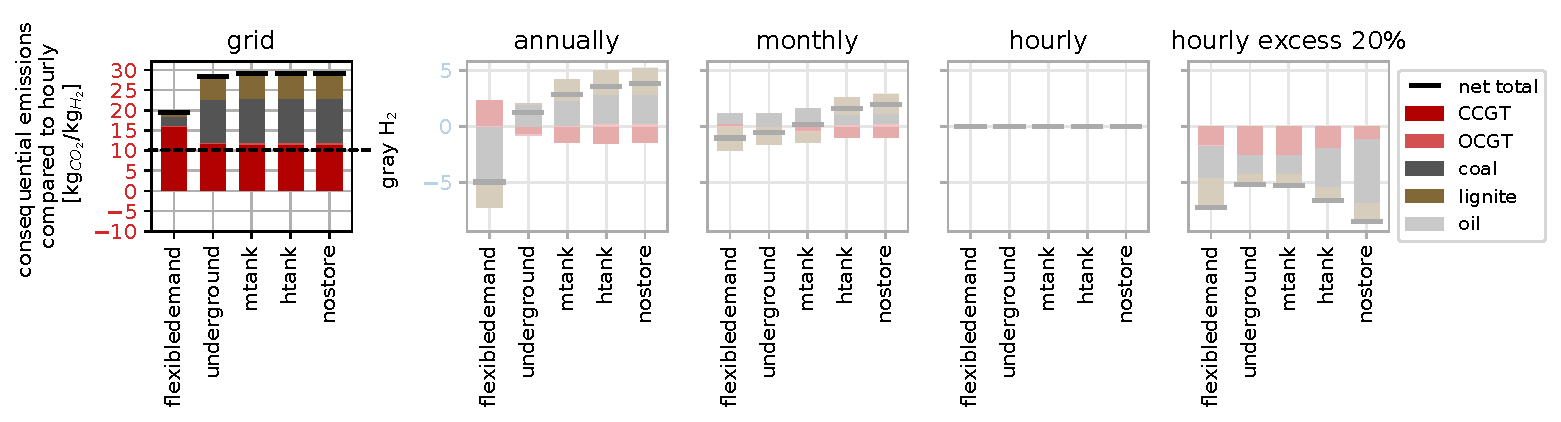
\includegraphics[width=1\linewidth]{images/consequential_emissions_by_carrier_3200wmonthly_v1.pdf}
	\end{figure}
	\begin{itemize}
		\item \alert{Additional local procurement} is \alert{essential} to prevent emission increases
		%		\item \alert{Hourly matching} with excess sales offers the \alert{most significant emission reductions}
	\end{itemize}
\end{frame}

\begin{frame}{Results - Emission Impacts of Hydrogen Production: Germany 2025}
	\addtocounter{framenumber}{-1}
	\begin{figure}
		\centering
		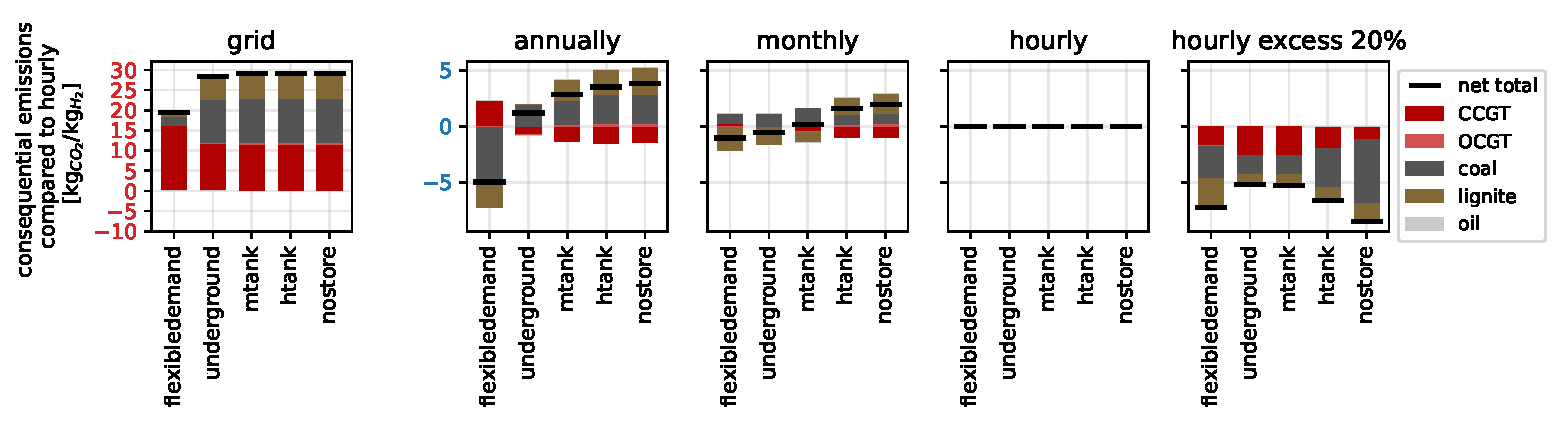
\includegraphics[width=1\linewidth]{images/consequential_emissions_by_carrier_3200wmonthly.pdf}
	\end{figure}
	\begin{itemize}
		\item \alert{Additional local procurement} is \alert{essential} to prevent emission increases
		\item The effects of annual and monthly matching are complex: \alert{flexible operations reduce} emissions, but \alert{constant} operations \alert{increase} them
		%		\item \alert{Hourly matching} with excess sales offers the \alert{most significant emission reductions}
	\end{itemize}
\end{frame}

\begin{frame}{Results - Hydrogen Production Costs: Germany 2025}
	\begin{figure}
		\centering
		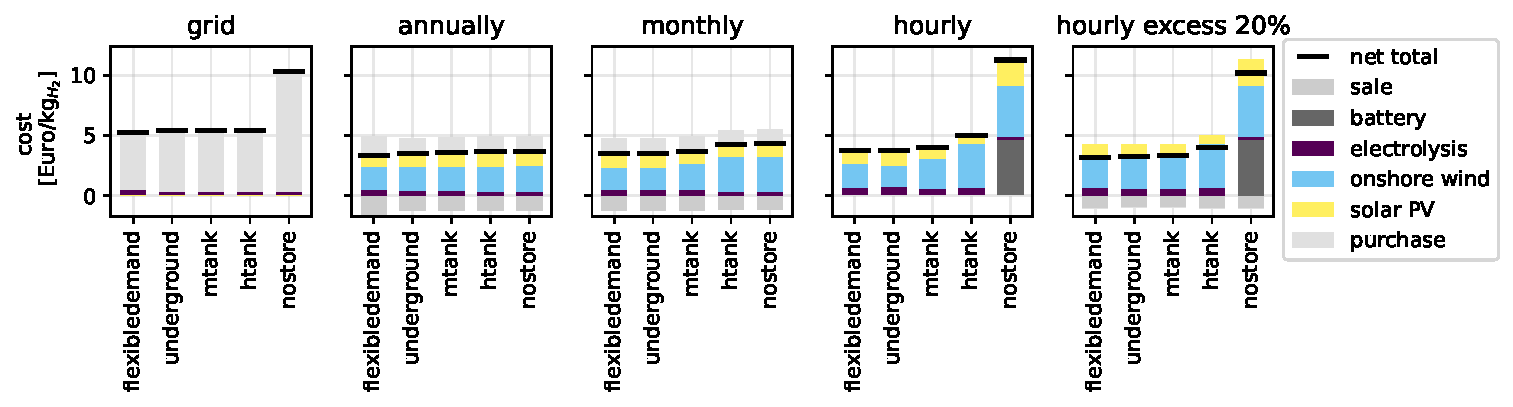
\includegraphics[width=1\linewidth]{images/costbreakdown_3200wmonthly.pdf}
		\label{fig:costbreakdown3200}
	\end{figure}
	\alert{Small Cost Premium}: Hourly matching has a 7--8\% cost premium over annual matching, given low-cost hydrogen storage or flexible demand
\end{frame}

\begin{frame}{Comparing Hydrogen Production in Carbon-Intensive vs. Clean Grids}
	\begin{figure}
		\centering
		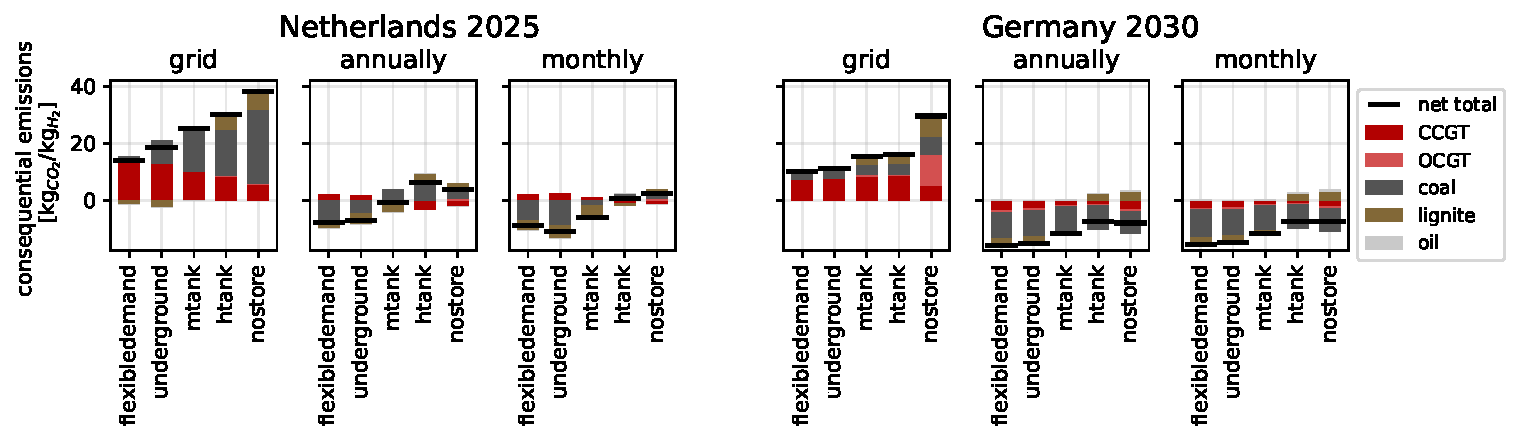
\includegraphics[width=0.9\linewidth]{../../../hourly_vs_annually/results/gas_price_35_nocrossover/graphs/consequential_emissions_by_carrier_3200_cleanness}
	\end{figure}
	\begin{columns}[T]
		\begin{column}{0.48\textwidth}
			\centering
			\textbf{Lower RES share of 49\%} \\
			\alert{Emissions} can \alert{rise} to nearly \alert{4x} the intensity of \alert{grey hydrogen}.
%			\begin{itemize}
%				\item \alert{Emissions} can \alert{rise} to nearly \alert{4x} the intensity of \alert{grey hydrogen}.
%				\item \alert{Annual/monthly matching} can \alert{reduce emissions} with \alert{flexibility}. However, with \alert{costly storage}, they may \alert{rise} by up to 6\kgco.
%			\end{itemize}
		\end{column}
		
		\begin{column}{0.48\textwidth}
			\centering
			\textbf{Higher RES share of 80\%} \\
			With \alert{higher decarbonisation}, temporal \alert{regulation} of hydrogen production matters \alert{less}.
%			\begin{itemize}
%				\item \alert{Emissions drop} in \alert{all} scenarios with \alert{additional} local RES.
%				\item With \alert{higher decarbonisation}, temporal \alert{regulation} of hydrogen production matters \alert{less}.
%			\end{itemize}
			
		\end{column}
	\end{columns}
\end{frame}

\begin{frame}{Take Aways - Temporal Regulation of Green Hydrogen Production}
	\begin{tcolorbox}[colback=white!5,colframe=white!60!black,title=\textbf{Green hydrogen certification: Low emissions \& low costs require}]
		\begin{columns}[t]
			\begin{column}{0.7\textwidth}
				%\begin{enumerate}
				
\includegraphics[width=0.09\linewidth]{images/res} Additional local renewable generation  \\
				\vspace{0.2cm}
				
\includegraphics[trim={0 0.5cm 0 0}, clip, width=0.05\linewidth]{images/clock} Temporal matching either
				\begin{itemize}
					\item Hourly with flexible demand or low-cost storage
					\item Annual with limited electrolysis full load hours
					\item Annual with a largely decarbonised background grid
				\end{itemize}
				%\end{enumerate}
			\end{column}
			\begin{column}{0.3\textwidth}
				\begin{figure}
					\vspace{-0.5 cm}
					\centering
					
\includegraphics[width=0.5\linewidth]{images/greenh2}
				\end{figure}
				
			\end{column}
		\end{columns}
	\end{tcolorbox}
	\textbf{Further interesting insights:}
	\begin{itemize}
		\item High dependency of consequential emissions on the background system
		\item Impact on how additionality is modelled
	\end{itemize}
\end{frame}

\section{24/7 Carbon-Free Electricity}
% New study released: here we explore the value of demand flexibility for 24/7 CFE
\begin{frame}{New study: The value of space-time load-shifting flexibility \\ 
  for 24/7 carbon-free electricity procurement (July 2023)}
  
    {\small
    \begin{columns}
    \begin{column}{9cm}
    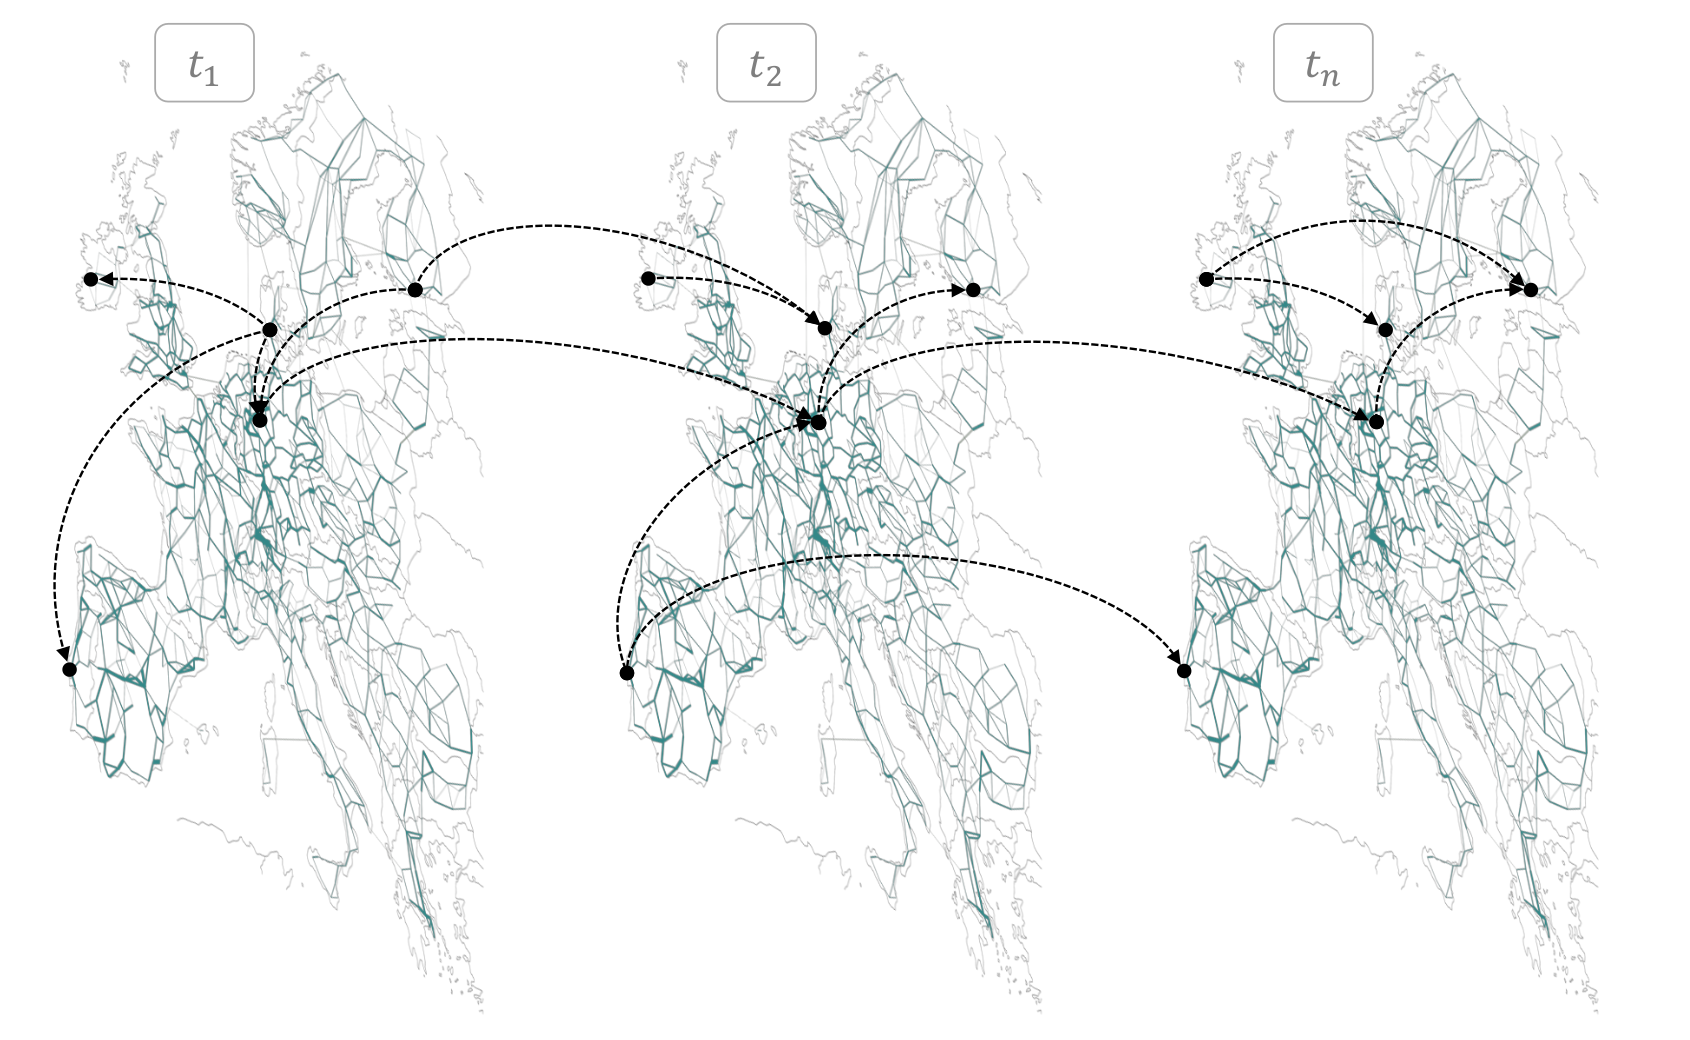
\includegraphics[width=10cm]{images/spatial-temporal-vlinks-cropped.png}
    \end{column}
  
    \begin{column}{6cm}
  
    \begin{itemize}
      \vspace{-0.2cm}
       \item Key focuses: \\
     -- How can demand flexibility reduce the required \alert{resources} and \alert{costs} of 24/7~CFE matching?\\ 
     \vspace{0.1cm}
     -- What are the \alert{signals} for optimal utilisation of demand flexibility?\\
     \vspace{0.1cm}
     -- What are the trade-offs and synergies from co-optimisation of \alert{spatial} and \alert{temporal} load shifting?
  
     \item Open-access research: \\
     \vspace{0.2cm}
     {\footnotesize
     \faUnlock~study:
     \hrefc{https://zenodo.org/records/8185850}{zenodo.org/records/8185850}\\
     \faUnlock~code:
     \hrefc{https://github.com/PyPSA/247-cfe}{github.com/PyPSA/247-cfe}\\
     }

     \item  A follow-up research paper to be released in March 2024.
  
    \end{itemize}
    \end{column}
    \end{columns}
    }
  \end{frame}
  
  
  % Brief overview of the study design
  \begin{frame}{Methods and study design}
  
    {\footnotesize
    \begin{columns}
    \begin{column}{9cm}
    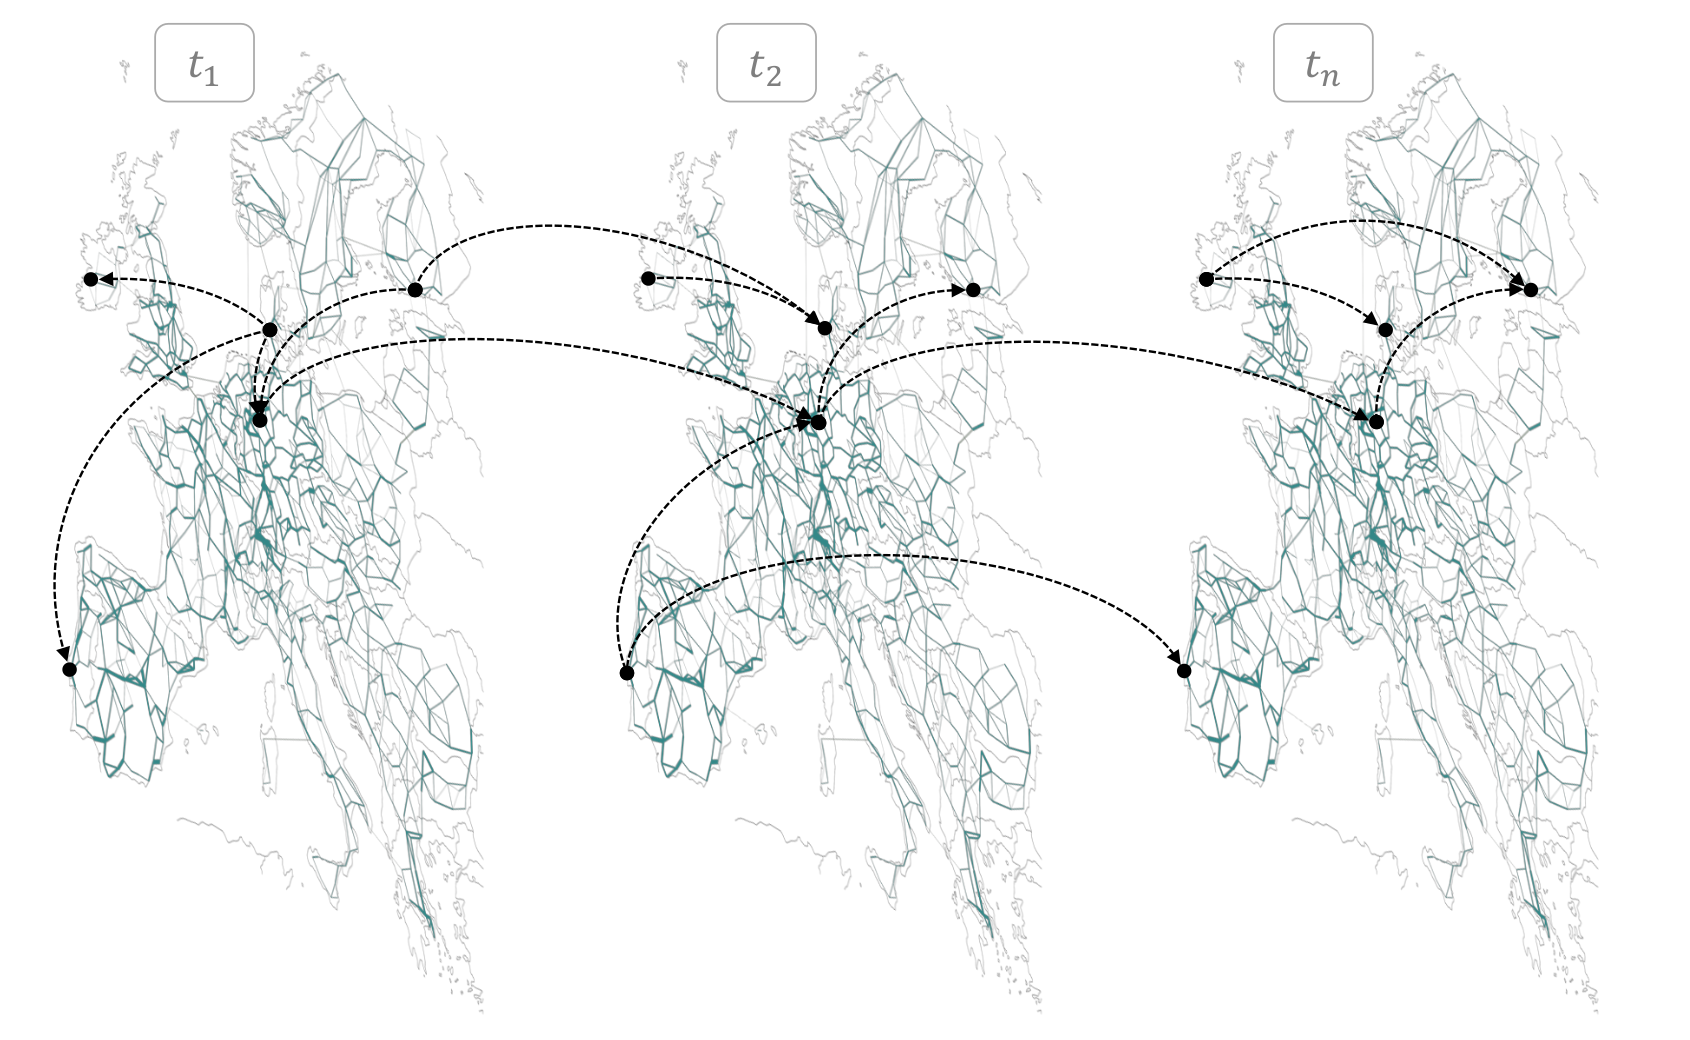
\includegraphics[width=10cm]{images/spatial-temporal-vlinks-cropped.png}
    \end{column}
  
    \begin{column}{6cm}
      \begin{itemize}
        \vspace{-0.1cm}
        \item The study is done with \alert{PyPSA} -- an open-source framework for modelling modern energy systems.
        \item Model scope: \alert{\href{https://www.entsoe.eu/data/map/}{ENTSO-E area}} power system clustered to individual bidding zones, \alert{hourly} temporal resolution. 
        \item Geographically scattered datacenters that are managed collectively. An operating company follows \alert{24/7 CFE strategy} in all locations.
        \item \alert{Spatial} and \alert{temporal} load shifting mechamisms.
        \item \alert{\enquote{Flexible workloads}}, i.e. electricity loads that can potentially be shifted in space or in time, are assumed to be in a range of {\{0\% .. 40\%\}}.
      \end{itemize}
      \end{column}
      \end{columns}
    }
\end{frame}
  

\begin{frame}{Signal 1: quality of local renewable resouces}

  \centering
  \vspace{0.3cm}
  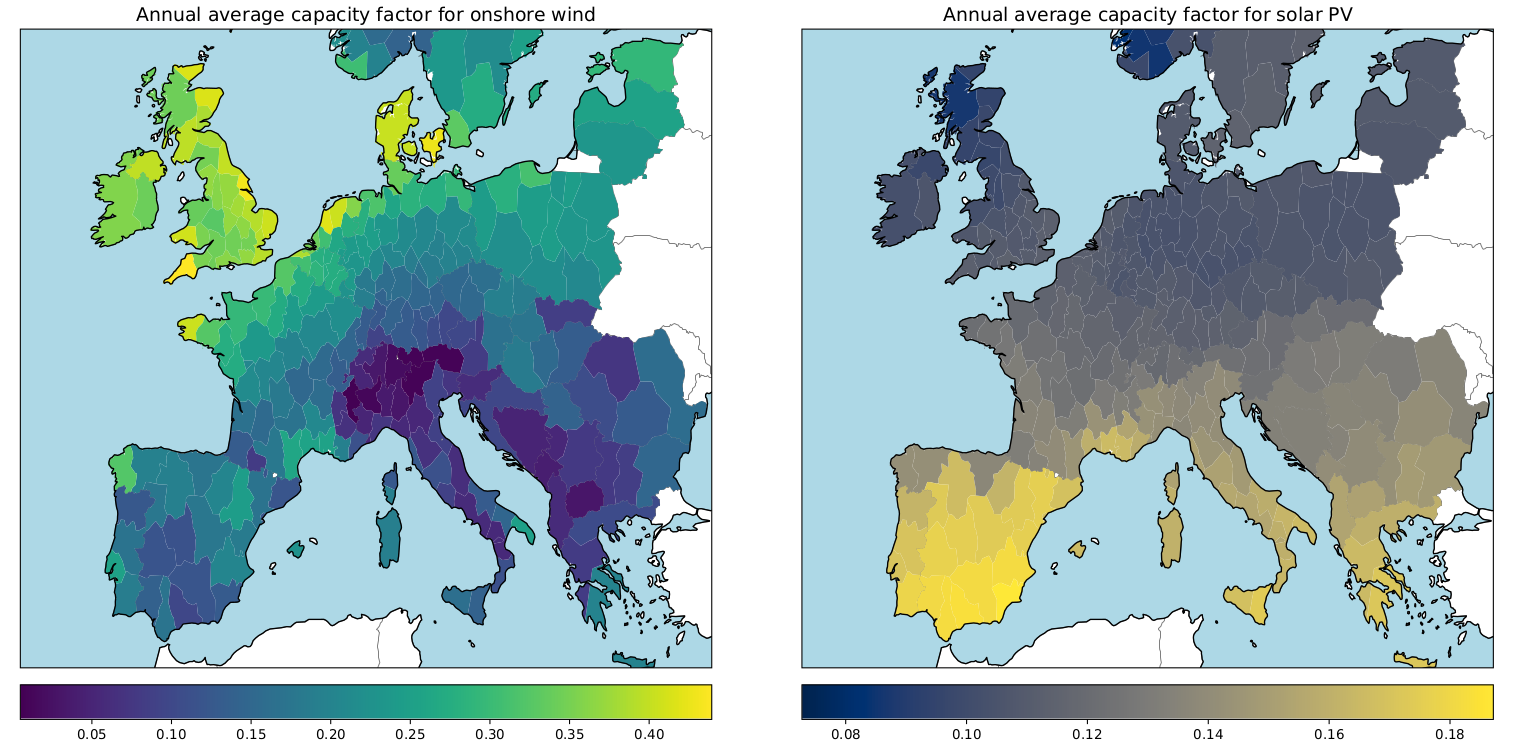
\includegraphics[width=14cm]{images/results-1.png}

\end{frame}


\begin{frame}{Signal 2: low correlation of wind power generation over long distances}
  \centering
  \vspace{0.3cm}
  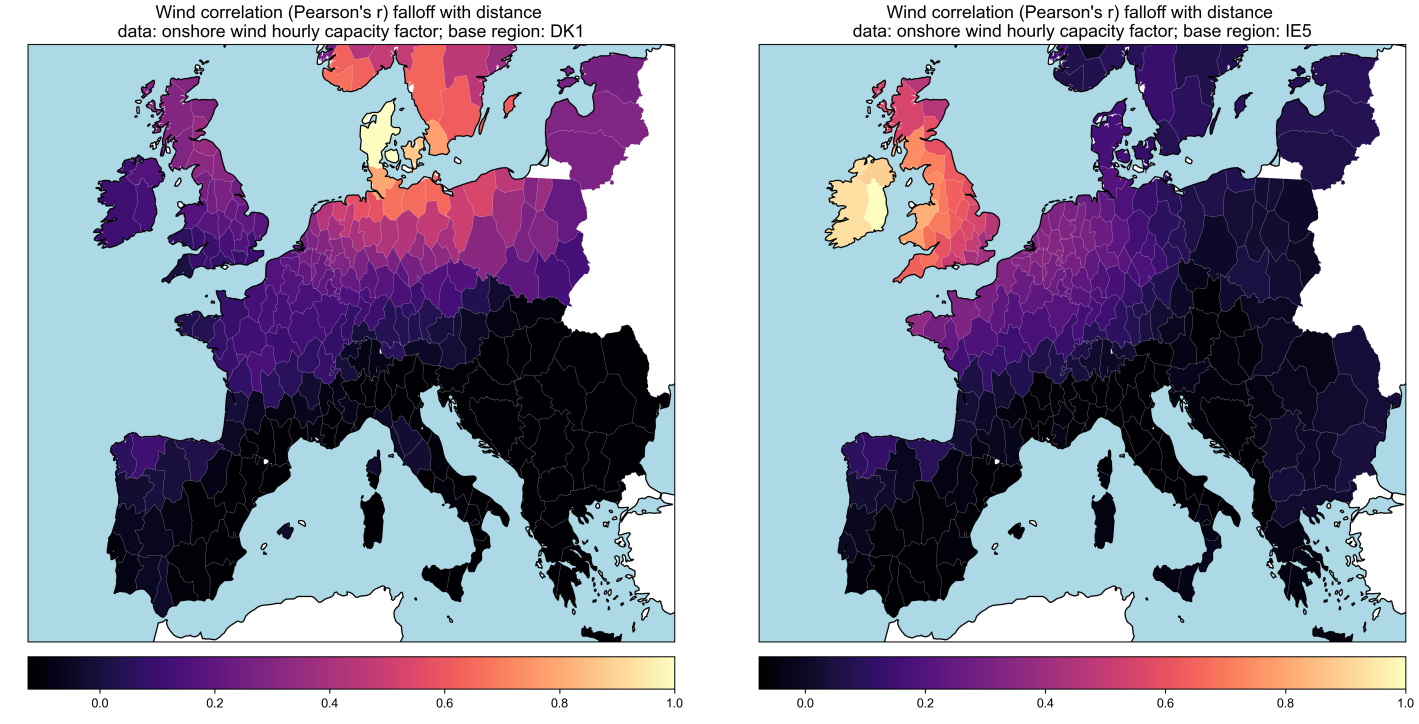
\includegraphics[width=14cm]{images/results-4.png}
\end{frame}


\begin{frame}{Cost savings as a function of distance between datacenter pair}
  \centering
  \vspace{0.3cm}
  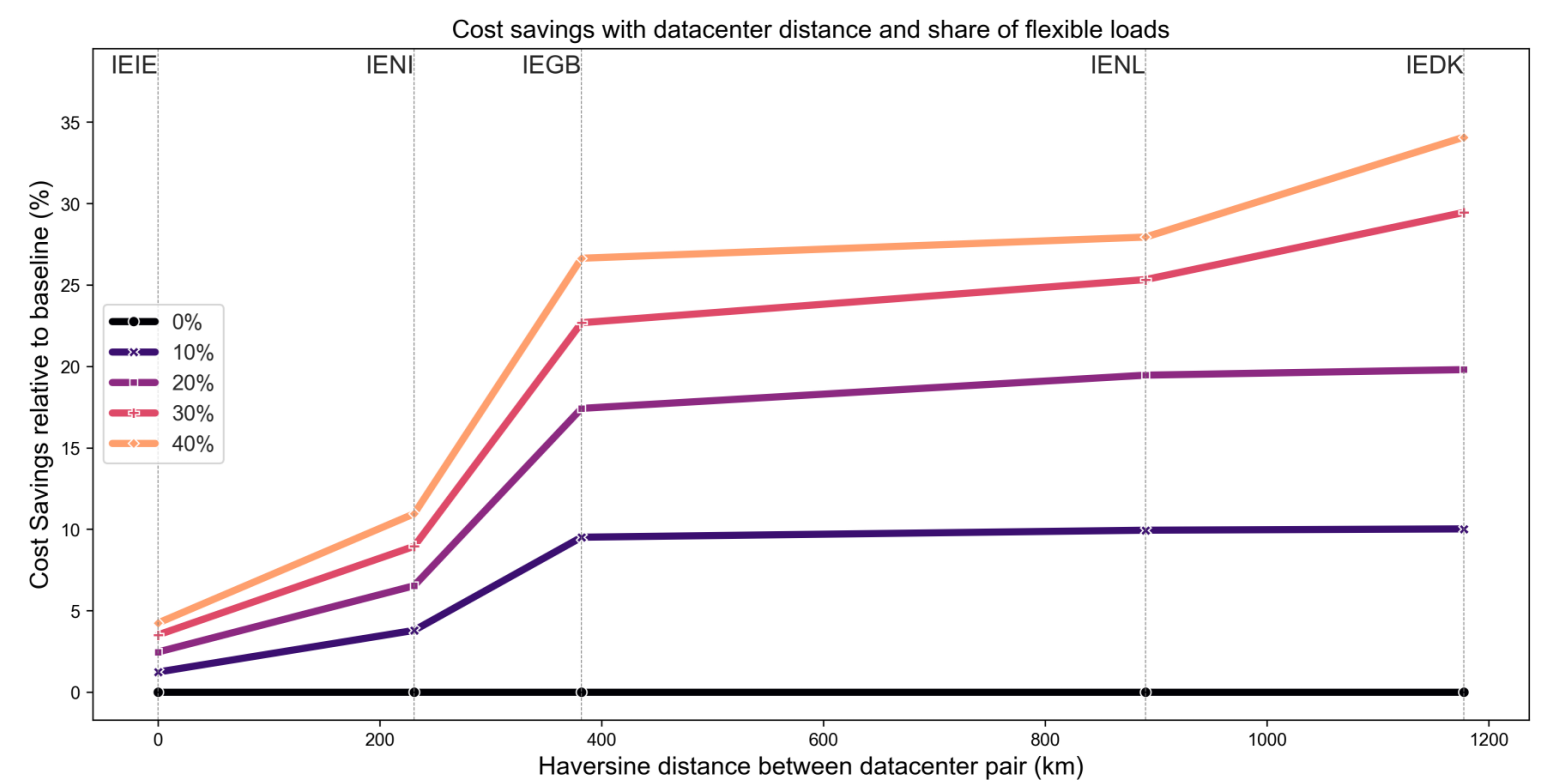
\includegraphics[width=14cm]{images/results-5.png}
\end{frame}


\begin{frame}{Time-series of optimized spatial load shifts (locations: DK-IE)}
  \centering
  \vspace{0.3cm}
  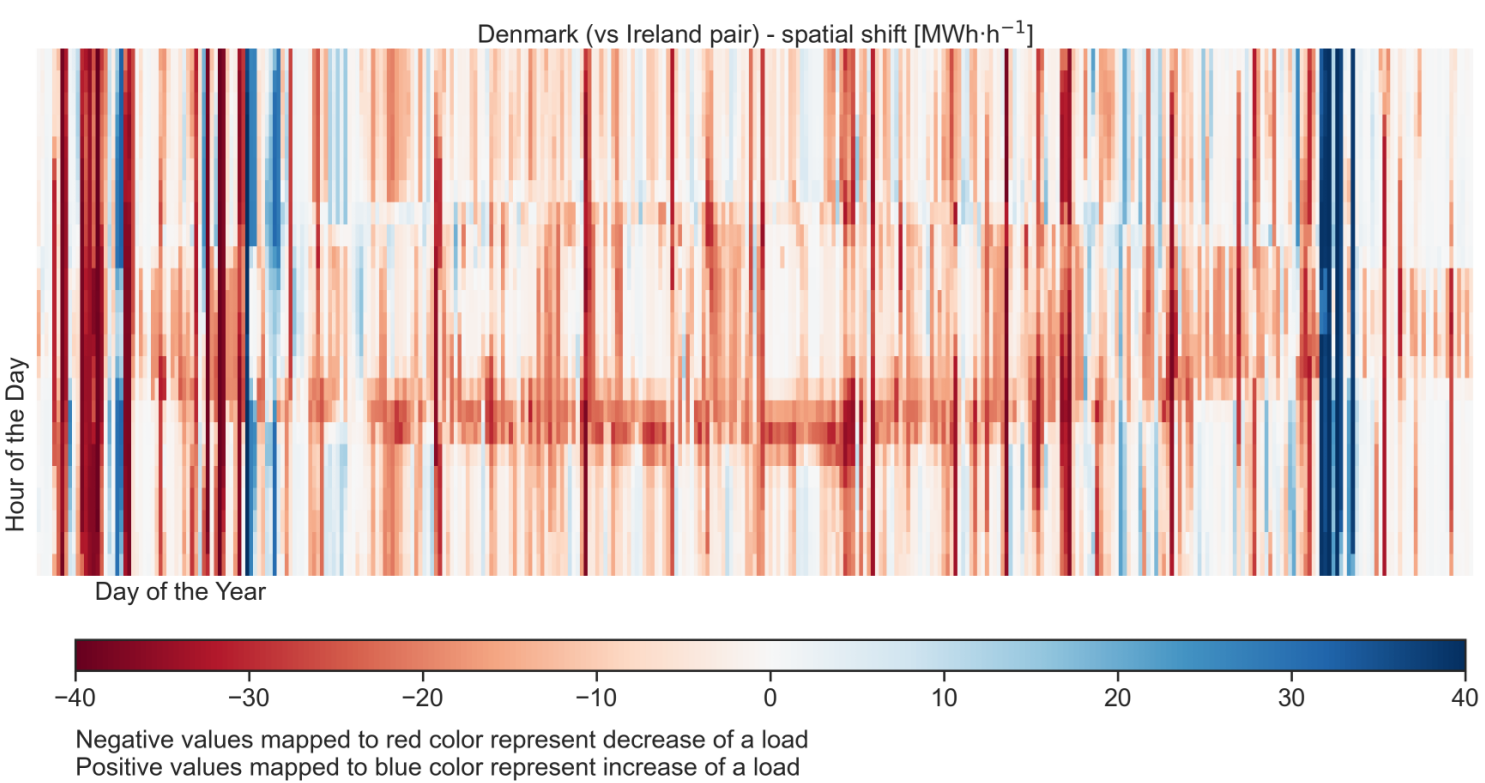
\includegraphics[width=14cm]{images/results-6.png}
\end{frame}


\begin{frame}{Signal 3: time lag in solar radiation peaks due to Earth's rotation (1/2)}
  \centering
  \vspace{0.3cm}
  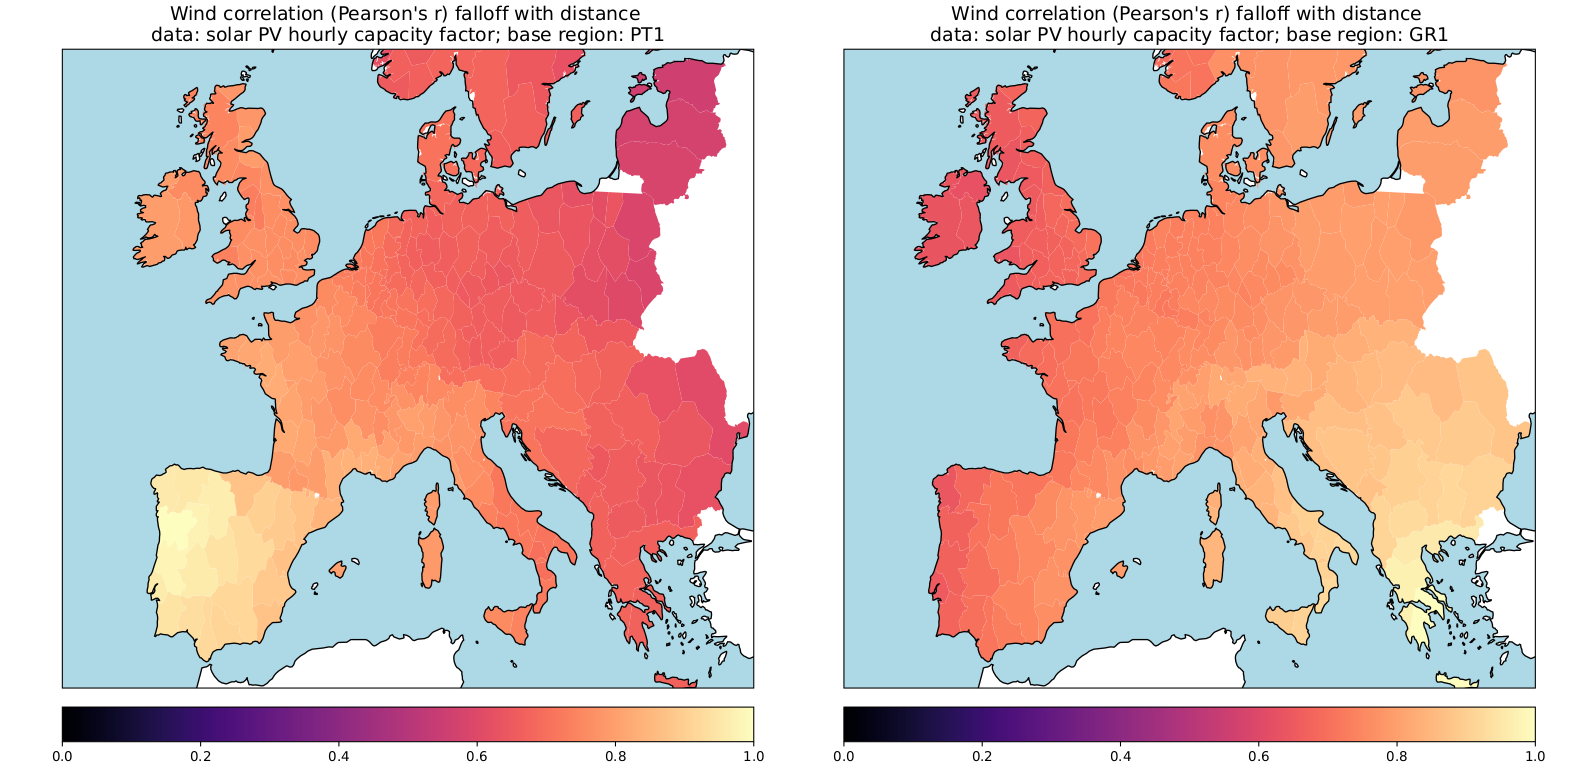
\includegraphics[width=14cm]{images/results-7.png}
\end{frame}


\begin{frame}{Signal 3: time lag in solar radiation peaks due to Earth's rotation (2/2)}
  \centering
  \vspace{0.3cm}
  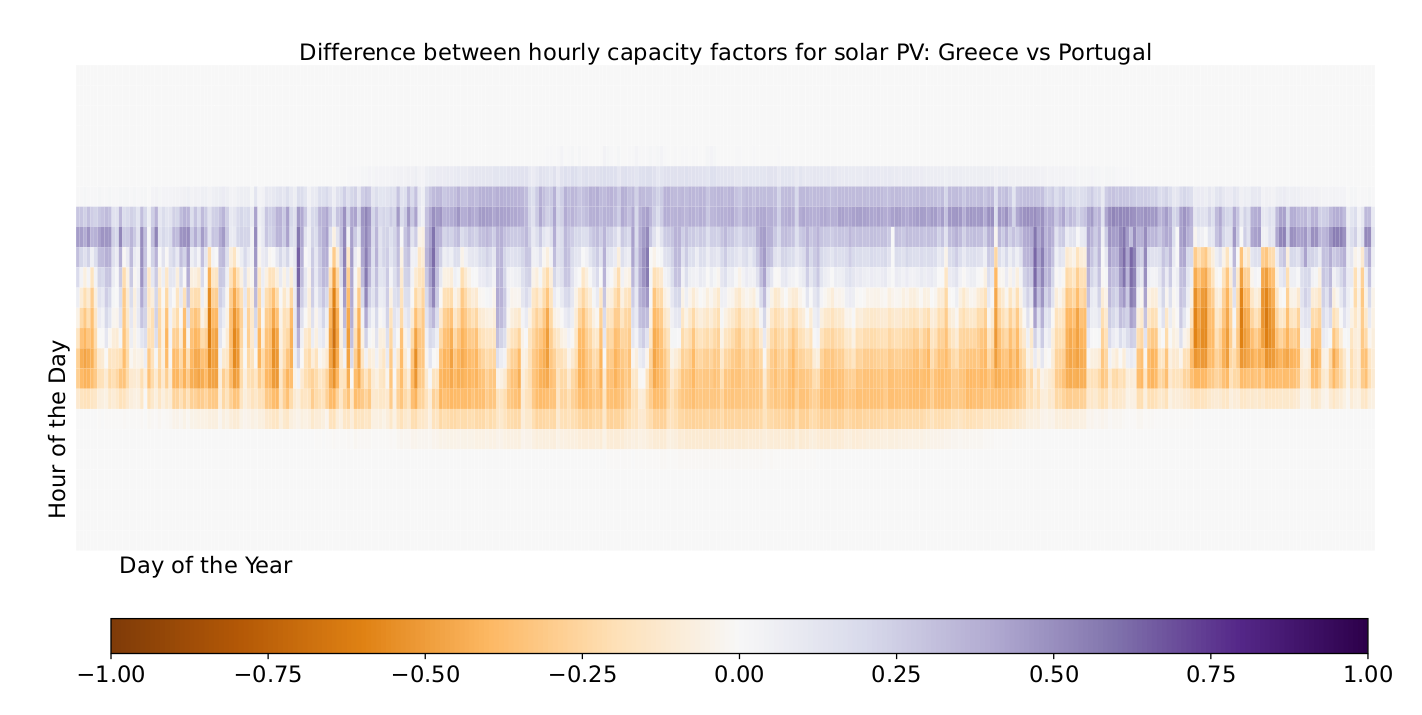
\includegraphics[width=14cm]{images/results-8.png}
\end{frame}



\begin{frame}{Also in the study}
  
      \begin{itemize}
      \item Scenarios for \alert{co-optimised} and \alert{isolated} utilisation of space-time load-shifting;
      \item Scenarios for 24/7 CFE with \alert{98\% and 100\%} matching targets;
      \item Scenarios with different \alert{24/7 technology options} (e.g., Long Duration Energy Storage);
      \item 24/7 CFE \alert{cost breakdowns} and \alert{procurement strategies} for individual locations;
      \item \alert{Synergies} and \alert{trade-offs} between spatial and temporal load shifting;
      \item Analysis of \alert{net load migration} across locations;
      \item Simulated \alert{energy balances} for selected datacenters.
      \end{itemize}

\end{frame}

\begin{frame}{Take aways}

There are \alert{three signals} companies can factor into their procurement \& load shaping strategies for 24/7 CFE matching: \\
\vspace{0.1cm}
  -- quality of local renewable resources;\\
  -- low correlation of wind power generation over long distances;\\
  -- time lag in solar radiation peaks due to Earth's rotation.\\

\vspace{0.5cm}

Overall, space-time load-shifting flexibility: \\
\vspace{0.1cm}
  -- enables \alert{better access to clean electricity} and creates \alert{more options} for consumers to match demand with carbon-free electricity around-the-clock; \\
  -- \alert{lowers the costs} of 24/7 CFE matching and makes it \alert{more attractive} to a wider range of companies.\\

    
\end{frame}


%----------------------------------------
%----------------------------------------

\begin{frame}\frametitle{\quad}

  {\Large
  \alert{Contacts, Resources, Acknowledgements}
  }

  \vspace{0.1cm}
    
  {\bf References:}
  \hrefc{https://iopscience.iop.org/article/10.1088/1748-9326/ad2239}{Temporal regulation of renewable supply for electrolytic hydrogen (2023)}\\
  {\bf References:} \hrefc{https://irieo.github.io/247cfe.github.io/}{More about the 24/7 CFE research project (2022-2024)}

  {\bf Code:} This work done in a spirit of open and reproducible research: \\
  \faUnlock~code:
  \hrefc{https://github.com/PyPSA/247-cfe}{github.com/PyPSA/247-cfe} \\
  \faUnlock~code: \hrefc{https://zenodo.org/records/8324521}{https://zenodo.org/records/8324521}
  
  \vspace{.1cm}
  {\bf Copyright:} Unless otherwise stated, graphics and text are Copyright \copyright E.Z. and I.R. 2024. \\
  This work is licensed under a \href{https://creativecommons.org/licenses/by/4.0/}{CC BY 4.0}.  {\footnotesize \ccby} 

  \vspace{.1cm}
  {\bf Send an email:} \\
  Dr. Elisabeth Zeyen, e.zeyen@tu-berlin.de\\
  Dr. Iegor Riepin, iegor.riepin@tu-berlin.de \\
  
\end{frame}


%%%%%%%%%%%%%%%%%%%%%%%%%%%%%%%%%%%%%%%%%%%%%%%%%%%%%%
\end{document}
%%%%%%%%%%%%%%%%%%%%%%%%%%%%%%%%%%%%%%%%%%%%%%%%%%%%%%